% File SDSS2020_SampleExtendedAbstract.tex
\documentclass[10pt]{article}\usepackage[]{graphicx}\usepackage[]{color}
% maxwidth is the original width if it is less than linewidth
% otherwise use linewidth (to make sure the graphics do not exceed the margin)
\makeatletter
\def\maxwidth{ %
  \ifdim\Gin@nat@width>\linewidth
    \linewidth
  \else
    \Gin@nat@width
  \fi
}
\makeatother

\definecolor{fgcolor}{rgb}{0.345, 0.345, 0.345}
\newcommand{\hlnum}[1]{\textcolor[rgb]{0.686,0.059,0.569}{#1}}%
\newcommand{\hlstr}[1]{\textcolor[rgb]{0.192,0.494,0.8}{#1}}%
\newcommand{\hlcom}[1]{\textcolor[rgb]{0.678,0.584,0.686}{\textit{#1}}}%
\newcommand{\hlopt}[1]{\textcolor[rgb]{0,0,0}{#1}}%
\newcommand{\hlstd}[1]{\textcolor[rgb]{0.345,0.345,0.345}{#1}}%
\newcommand{\hlkwa}[1]{\textcolor[rgb]{0.161,0.373,0.58}{\textbf{#1}}}%
\newcommand{\hlkwb}[1]{\textcolor[rgb]{0.69,0.353,0.396}{#1}}%
\newcommand{\hlkwc}[1]{\textcolor[rgb]{0.333,0.667,0.333}{#1}}%
\newcommand{\hlkwd}[1]{\textcolor[rgb]{0.737,0.353,0.396}{\textbf{#1}}}%
\let\hlipl\hlkwb

\usepackage{framed}
\makeatletter
\newenvironment{kframe}{%
 \def\at@end@of@kframe{}%
 \ifinner\ifhmode%
  \def\at@end@of@kframe{\end{minipage}}%
  \begin{minipage}{\columnwidth}%
 \fi\fi%
 \def\FrameCommand##1{\hskip\@totalleftmargin \hskip-\fboxsep
 \colorbox{shadecolor}{##1}\hskip-\fboxsep
     % There is no \\@totalrightmargin, so:
     \hskip-\linewidth \hskip-\@totalleftmargin \hskip\columnwidth}%
 \MakeFramed {\advance\hsize-\width
   \@totalleftmargin\z@ \linewidth\hsize
   \@setminipage}}%
 {\par\unskip\endMakeFramed%
 \at@end@of@kframe}
\makeatother

\definecolor{shadecolor}{rgb}{.97, .97, .97}
\definecolor{messagecolor}{rgb}{0, 0, 0}
\definecolor{warningcolor}{rgb}{1, 0, 1}
\definecolor{errorcolor}{rgb}{1, 0, 0}
\newenvironment{knitrout}{}{} % an empty environment to be redefined in TeX

\usepackage{alltt}
\usepackage{newtxtext, newtxmath, times}
\usepackage{sdss2020} % Uses Times Roman font (either newtx or times package)
\usepackage{url}
\usepackage{latexsym}
\usepackage{amsmath, amsfonts}
\usepackage{algorithm, algorithmic}  
\usepackage{graphicx}
\usepackage[dvipsnames]{xcolor} % colors

% Commands for editing
\newcommand{\db}[1]{{\textcolor{orange}{#1}}}
\newcommand{\svp}[1]{{\textcolor{blue}{#1}}}

%\title{Symposium on Data Science and Statistics (SDSS 2022) \\
%Submission and Formatting Instructions for Extended Abstracts}

\title{Exploring Rural Shrink Smart Through Guided Discovery Dashboards}

\author{
  Denise Bradford \\
  University of Nebraska - Lincoln \\
  Lincoln, Nebraska \\
  {\tt denise.bradford@huskers.unl.edu} \\\And
  Susan VanderPlas \\
  University of Nebraska - Lincoln \\
  Lincoln, Nebraska \\
  {\tt susan.vanderplas@unl.edu} \\}
  

\date{}
\IfFileExists{upquote.sty}{\usepackage{upquote}}{}
\begin{document}




\maketitle
\begin{abstract}
Many small and rural places are shrinking. Interactive dashboards are the most common use cases for data visualization and context for exploratory data tools. In our paper, we will explore the specific scope of how dashboards are used in small and rural area to empower novice analysts to make data-driven decisions. Our framework will suggest a number of research directions to better support small and rural places from shrinking using an interactive dashboard design, implementation and use for the every day analyst. 
\end{abstract}

{\bf Keywords:} Interactive Dashboards, Exploratory Data Analysis (EDA), Guided Discovery

\section{Research Problem}
With the amount of publicly open-source data, a proliferation of visualization dashboards has increased in nearly every industry \cite{fisher}. A dashboard in its fundamental form, a dashboard supports a way of presenting and making sense of complex data to better enable and support decision making. Stephen Few defines a dashboard as:

\begin{quotation}% I don't know that we need this... dashboards are very common, so let's focus on the problem and the dashboard as an obvious solution.
\small A visual display of the most important information needed to achieve one or more objectives, consolidated and arranged on a single screen so the information can be monitored at a glance. \cite{few}
\end{quotation}

Some communities continue to thrive as they lose population because they adapt\svp{, maintaining quality of life and community services for residents while} investing in the future. % putting sentences on different lines helps with git merges and also makes it easier to figure out where {} match up :)
\svp{This process,} \emph{smart shrinkage}\svp{, is important for rural areas who have experienced shrinking populations for decades.} 
\svp{As small rural towns do not have access to data scientists or even the ability to easily leverage data collected locally to support decisions, our} research team \svp{will provide communities with data about services in small town Iowa in order to assist with} developing strategies to improve quality of life for their residents amid shrinking populations \cite{scc}. \svp{We hope to allow towns to discover their own data and compare to other similar towns, centering decision-making on data in the context of small-town Iowa life. In the process, we will assess our visualizations to determine which strategies for user interface and interactive graphics design are most useful to empower town leaders to make discoveries in publicly available data assembled with a focus on items that impact rural quality of life.}
% Our work focuses on developing and challenges novice analysts in advanced statistical concepts and data visualizations to help make decisions. Specifically, what data can be used to help make decisions, what strategies overcome the challenges of those analysts feel empowered to make data-driven decisions. Our ultimate aim is to help inform Iowa's Rural Shrink Smart communities by using effective dashboards to help those towns build the Quality of Life (QoL) Measures.

\section{Data Description}
\svp{Data collected from \url{data.iowa.gov}} were used to create the SCC dashboard. \svp{Most of these datasets are collected on a town/city or county level, requiring us to carefully join data accounting for differences in spatial resolution.} \svp{\url{data.iowa.gov} contains unique information about residents, including local liquor sales, school building locations, town budgets and expenditures, hospital beds, Medicaid reimbursements, and other details that may provide information about local quality of life.} 
\svp{Using this data, we created a dashboard which allows communities to explore these data and compare and contrast their local community to other communities of similar size and location. In addition to manual comparisons created by the user, we will use statistical clustering methods to identify groups of towns which employ similar strategies to maintain resident quality of life.}

\svp{One of the interesting features of this assembled dataset is that missing data can be missing for multiple reasons: not all state data is complete, but data about certain services may also be missing because towns do not offer that service.}
\svp{Thus, in addition to the usual challenges of working with real-world data that is "messy" in a variety of ways, we also have to contend with missing data that is missing due to the size of the community or the lack of services. This makes both visualization and statistical analysis more complicated.}

\section{Guiding Design Principles}
\svp{An additional challenge is that research on dashboard creation and interactive visualization tends to be very task-specific and not generalizable. That is, it is relatively easy to create a dashboard that works for a particular task, but it is hard to generalize from that process what will work for the next dashboard. With this in mind, we have clearly documented our intentions at each stage of the design and evaluation process, with the goal of gathering some useful information about general dashboard design from the process of creating this specific dashboard.}
\svp{Thus, our initial set of dashboard design principles is as follows: }
\begin{itemize}
\item \svp{The town leaders are the focus audience; thus, the town itself should be the central focus of the app.}
\item \svp{Facilitate comparisons with other towns in order to allow the user to explore other potential solutions to offering services that enhance resident quality of life.}
\item \svp{Present the user with peer comparisons in order to widen the scope of exploration beyond the initial set of obvious peers in the local region.}
\item \svp{Allow for more detailed data and feature requests to improve the dashboard design over time.}
\end{itemize}


\section{Current Progress and Future Work}
Our current design work will be broken down into four categories that have been identified in the following:
\begin{itemize}
\item User Flexibility 
\item Visual, Analytic, and Data Literacy
\item Data Design
\item Social Impact
\end{itemize}

In Figure 1, our dashboard will allow the user to select a town name, which will populate the  information in the maps related to necessary services, which include directions and distance to fire department, schools, post offices and hospitals. A table will be populated that will include information related to five other towns that have similar attributes, but the aspect of QoL will be included in the differences that help the town make a decision for the town. 

\begin{figure}[ht!]
\centering
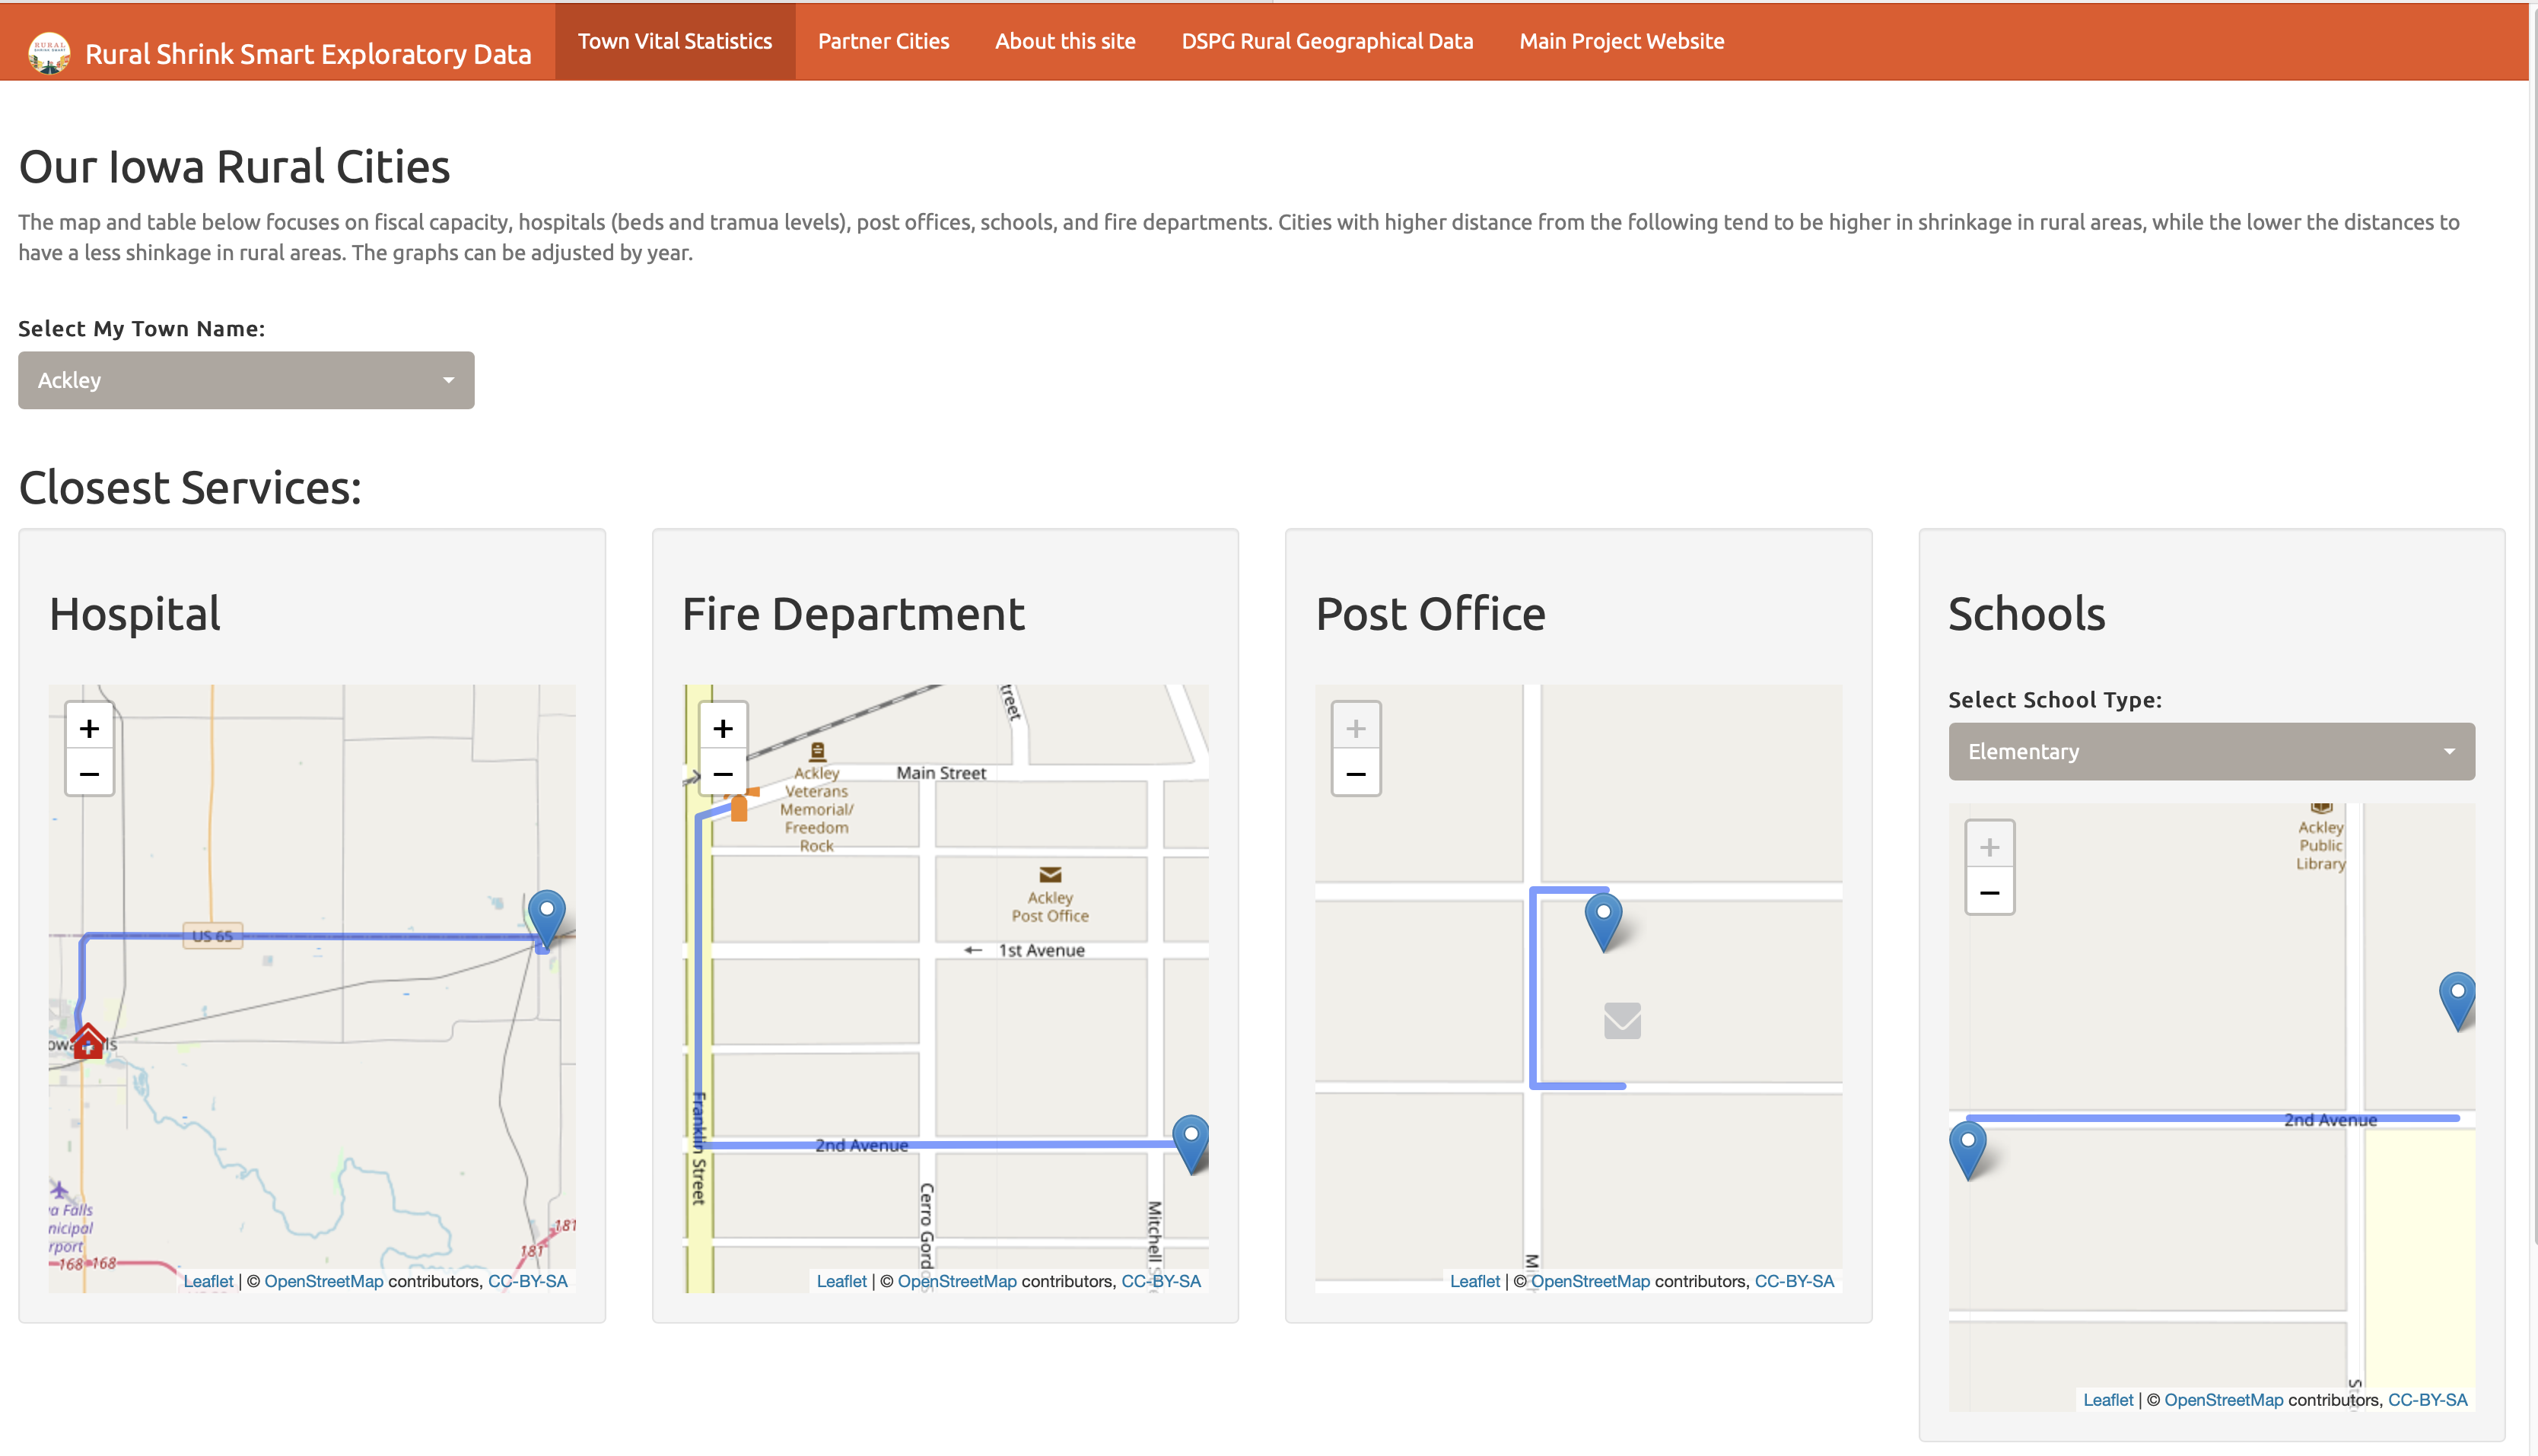
\includegraphics[width=75mm]{SCC_Dashboard.png}
\caption{Rural Smart EDA Dashboard Design}
\end{figure}


\subsection{Current Progress}
{\bf Statistical Techniques} Our research has incorporated statistical clustering methods, such as K-means and Hierarchical Clustering, to determine the similarities in the towns based on distances and services available. As a result, of our research partners we were actually able to use clustering methods to determine and identify missing data. We will continue to use clustering methods to identify the towns that will be best compare when the analyst interacts with our dashboard. 

{\bf Data Science Techniques} Our team has been able to utilize direct API calls and web scraping tools to collect data necessary.  

{\bf Dashboard Design Techniques} Our dashboard incorporates the following important dashboard techniques:
{\it User Flexibility} The aspects of user flexibility are directly based on the detail data adjustments; Adaptability: User and Display; Comparison support and Storytelling. For example, we want our users to use the data collected on a mass scale that have and should be summarized in detail but without losing anything.

{\it Visual, Analytic, and Data Literacy} The aspects in our dashboard development primary presents in our ability to ease of usage to the user with visual, data  and analytic literacy. We have little information on the users' adaptability to data-driven decisions. 

{\it Data Design}. In our case, the challenges that arise in our dashboard will include data quality, data grouping, too much data, data sources, inaccurate data representation, and key performance indicators and metrics. For example, we have information from {\it Iowa Data} will have missing data can be pointed out by our users' that has not been captured by our data sources, this can be a recent closing of a school due to the pandemic.

{\it Social Impact} This aspect will be about making sure that the users are flexible to the following: data-driven thinking, technology resistance, dashboard aversion, and data sharing, security, and privacy. For example, we will encounter town users that will have the urge to compare their town to all types of towns that aren't similar. In our research, we will use statistical clustering methods and cater dashboard to show only towns that have similar components.

\subsection{Future Work}
Our dashboard design has created challenges that promote 

We have five towns that have agreed to partner with the project to help with identify the best practices that are useful in the Iowa small and rural towns. As a result to our dashboard development, we will develop a feedback loop from the analyst in these five towns that will help provide our team with useful notes that will be adaptive to all of the small towns in Iowa. As a contrast, we will researchers with an extensive understanding of the small towns to be used as a counter example of dashboard adaptability. Our research, should be a 

So dashboard challenges,
adaptation techniques, and user strategies are interconnected as
Figure 1 shows. The rationale is that if we are able to establish
a relationship between strategies to problems and we can detect
the strategies in real-time, we can adapt the user interface in realtime or in the next iteration. Then we can say that the adaption
techniques have a positive effect on the challenges.
\section{Acknowledgements}
We would like to thank our sponsors and grant provider NSF, LSAMP Inspire Program and Iowa League of Cities. We would like to thank our partners and team members at Iowa State University and University of Nebraska - Lincoln. We would like to thank the State of Iowa for providing Data along with our partners in the Rural Iowa communities.


\bibliographystyle{sdss2020} % Please do not change the bibliography style
\bibliography{SCCAbstract_SDSS2022}

\end{document}
